\documentclass[a4paper, 11pt]{report}
\usepackage{blindtext}
\usepackage[T1]{fontenc}
\usepackage[utf8]{inputenc}
\usepackage{titlesec}
\usepackage{fancyhdr}
\usepackage{geometry}
\usepackage{fix-cm}
\usepackage[hidelinks]{hyperref}
\usepackage{graphicx}
\usepackage{titlesec}

\usepackage[english]{babel}

\geometry{ margin=30mm }
\counterwithin{subsection}{section}
\renewcommand\thesection{\arabic{section}.}
\renewcommand\thesubsection{\thesection\arabic{subsection}.}
\usepackage{tocloft}
\renewcommand{\cftchapleader}{\cftdotfill{\cftdotsep}}
\renewcommand{\cftsecleader}{\cftdotfill{\cftdotsep}}
\setlength{\cftsecindent}{2.2em}
\setlength{\cftsubsecindent}{4.2em}
\setlength{\cftsecnumwidth}{2em}
\setlength{\cftsubsecnumwidth}{2.5em}

\titlespacing\section{0pt}{12pt plus 4pt minus 2pt}{0pt plus 2pt minus 2pt}
\titlespacing\subsection{0pt}{12pt plus 4pt minus 2pt}{0pt plus 2pt minus 2pt}

\begin{document}
\titleformat{\section}
{\normalfont\fontsize{15}{0}\bfseries}{\thesection}{1em}{}
\titlespacing{\section}{0cm}{0.5cm}{0.15cm}
\titleformat{\subsection}
{\normalfont\fontsize{13}{0}\bfseries}{\thesubsection}{0.5em}{}
\titlespacing{\section}{0cm}{0.5cm}{0.15cm}

%=============================================================================

\pagenumbering{Alph}
\begin{titlepage}
\begin{flushright}

\includegraphics[width=4cm]{Images/USyd.jpg}\\[2cm]
\end{flushright}
\center 
\textbf{\huge INFO1111: Computing 1A Professionalism}\\[0.75cm]
\textbf{\huge 2023 Semester 1}\\[2cm]
\textbf{\huge Self-Learning Report}\\[3cm]

\textbf{\huge Submission number: 1}\\[0.75cm]
\textbf{Github link: ??}\\[2cm]

{\large
\begin{tabular}{|p{0.35\textwidth}|p{0.55\textwidth}|}
	\hline
	{\bf Student name} & Deana Hamdan El Madi\\
	{\bf Student ID} & 520481770\\
	{\bf Topic} & JavaScript\\
	{\bf Levels already achieved} & -\\
	{\bf Levels in this report} & A and B \\
	\hline
\end{tabular}
}
\thispagestyle{empty}
\end{titlepage}
\pagenumbering{arabic}


%=============================================================================

\tableofcontents

%=============================================================================


\newpage
\section{Level A: Initial Understanding}
\vspace{5mm}
\subsection{Level A Demonstration}
To demonstrate my Level A understanding of JavaScript, I will:

- Embed JavaScript into a web-page

- Create functions in JavaScript

- Learn about scope in JavaScript


\subsection{Learning Approach}
I approached my learning by first seeking to understand the fundamentals of JavaScript. This included basic syntax, data types and control structures. An important step in my learning approach was to cultivate good habits, such as commenting my code and writing clear and concise functions. I sought a demonstration of this by experienced developers, to ensure I was using best practise in my work. 
I browsed various resources to find a teaching style I liked. Through this, I stumbled across "Frontend Simplified" which taught how JavaScript is applied in Frontend Development. Since I was only a beginner, I started by watching the JavaScript crash-course.
I also joined Frontend Simplified's programming Discord server. This proved to be a very useful step in my self-learning journey, as participating in an online community allowed me to ask questions and learn from other people. I was able to find mentors and accountability partners to help me stay on track as I navigated through the content.
The final element of my learning approach was to be patient. I understood that learning a new language takes time and effort. I tried to not get discouraged if I didn't understand something right away, and wasn't afraid to ask for help or take a break when I needed it.


\subsection{Challenges and Difficulties}
Embedding JavaScript into a web-page is what I found most difficult, as this is a concept I haven't encountered in other programming languages. I didn't have prior experience in browser coding, or writing code for an interface. Rather than just writing a program in a JavaScript file, I learnt how to add JavaScript code to the HTML code of a web-page so that the browser can interpret and execute the JavaScript code when the web-page loads.

Another challenging concept was scope. This was because there are many factors in JavaScript that affect where a variable can be accessed. Although I had previous knowledge about global and local scope, I was introduce to block scope. The most difficult concept to grasp was "hoisting". This involved variables being used before they are declared! Variable and function declarations are moved (or "hoisted") to the top of their respective scope before any code is executed.


\subsection{Learning Sources}

\begin{tabular}{|p{0.45\textwidth}|p{0.45\textwidth}|}
	\hline
	Learning Source & Contribution to Learning \\
	\hline
	MDN Web Docs\cite{MDN_HTML_JS} JavaScript documentation on how to use JavaScript within a web-page. & Documentation is an essential resource for developers and learners alike, and greatly enhanced my learning process. I used MDN Web Docs to learn the syntax and functionality of writing JavaScript within HTML, explore new features and integrations, and troubleshoot specific problems I encountered.  Additionally, the documentation includes best practices and conventions for writing efficient, clean, and readable code. This helped me write code that is consistent with industry standards and is easy to maintain and understand.\\
	\hline
	Frontend Simplified: JavaScript crash-course \cite{FES_JS_Crash_Course}, JavaScript Beginner Challenges\cite{FES_JS_Beginner}, JavaScript Medium Challenges\cite{FES_JS_Medium}, JavaScript Advanced Challenges\cite{FES_JS_Hard}, JavaScript Interview Questions 
 (Fundamentals) \cite{FES_JS_Interview}& The JavaScript crash-course provided a quick and comprehensive overview of the language syntax and functionality, to help me understand the basics of the language. I used the challenge questions to learn how to create functions in JavaScript and apply what I learnt in a practical way, helping me reinforce my understanding of the language and develop my problem-solving skills. \\
	\hline
	Udemy: The Modern JavaScript Bootcamp\cite{Udemy_JS_Course} & The specific videos I watched from this bootcamp related to variable scoping. JavaScript scoping rules can be complex and confusing, and watching a video on the topic allowed me to see examples in action. The instructor provided examples and demonstrations that help to illustrate the key points.\\
	\hline
\end{tabular}

\subsection{Application artifacts}
I learnt how to embed JavaScript into a web-page using a <script> tag (Figure 1). There is an alternate method of having a separate .js file that is referenced with an src attribute.

In the JavaScript code, I used the \emph{alert()} function. This displays a pop-up dialog box with a message and an OK button. The message can be a string or a variable that contains a string. The alert function is used to provide a quick message or notification to the user and interrupts the execution of the JavaScript code until the OK button is clicked.

I opened my \emph{hello.html} file in my local host, and the dialog box appeared with my message (Figure 2). I was therefore successful in embedding JavaScript in the web-page. 

Additionally, I used the \emph{console.log()} method to write a message to the browser's console (Figure 3). The console is a tool that allows developers to view and interact with the JavaScript code that runs on a web-page. It can be accessed by opening the developer tools in a browser and selecting the "Console" tab.

\begin{figure}[ht]
    \centering
    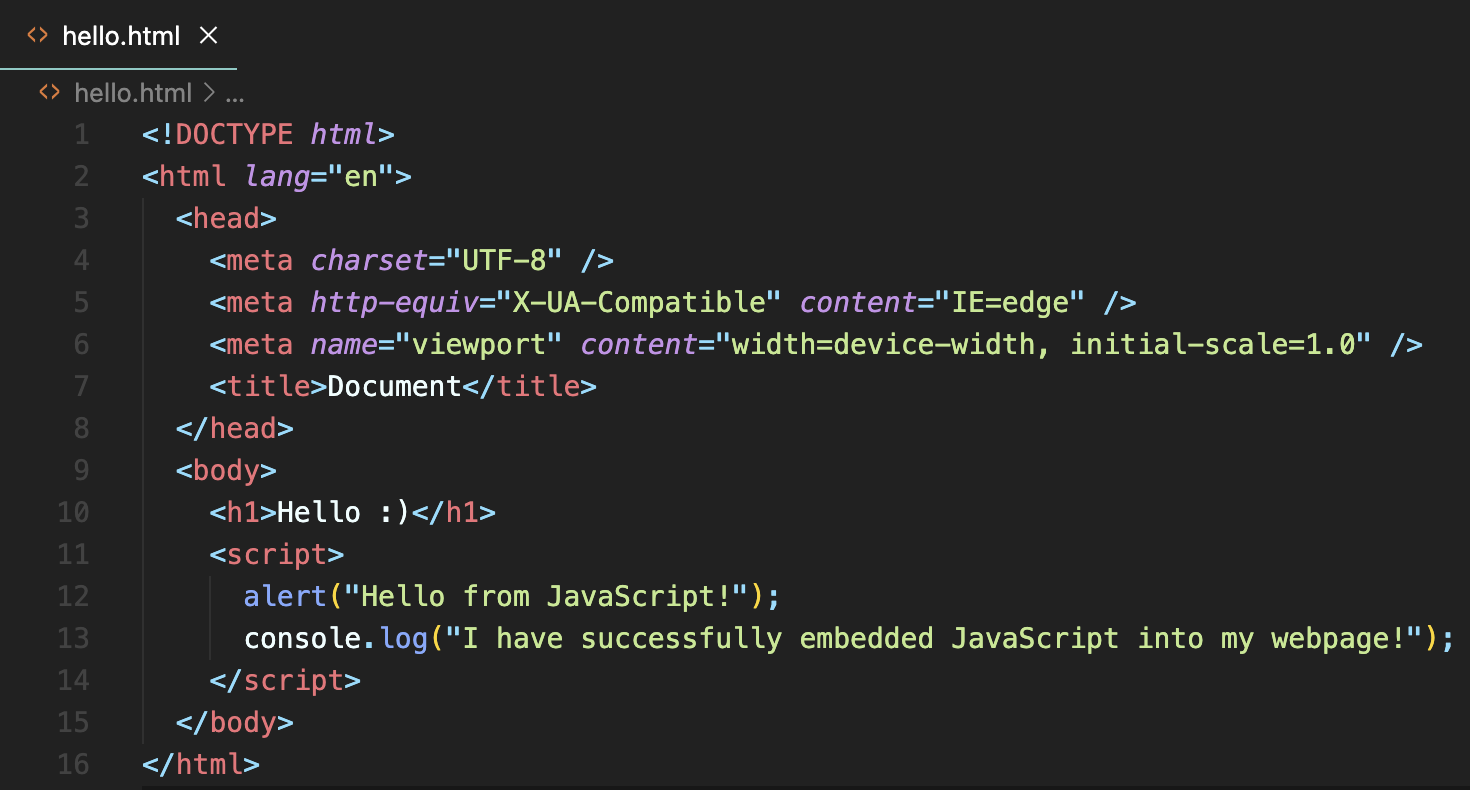
\includegraphics[width=0.8\textwidth]{Images/embedding1.png}
    \caption{Embedding JavaScript into a webpage}
    \label{fig:screenshot}
\end{figure}

\begin{figure}[ht]
    \centering
    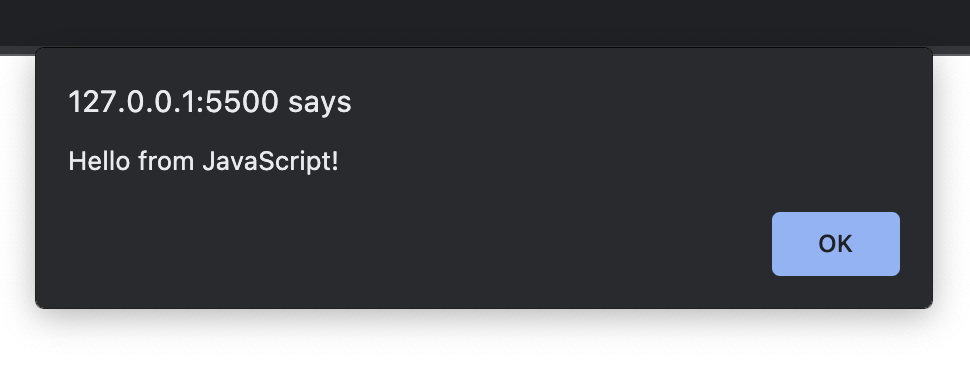
\includegraphics[width=0.8\textwidth]{Images/embedding2.png}
    \caption{Web-page's pop-up dialog box}
    \label{fig:screenshot}
\end{figure}

\begin{figure}[ht]
    \centering
    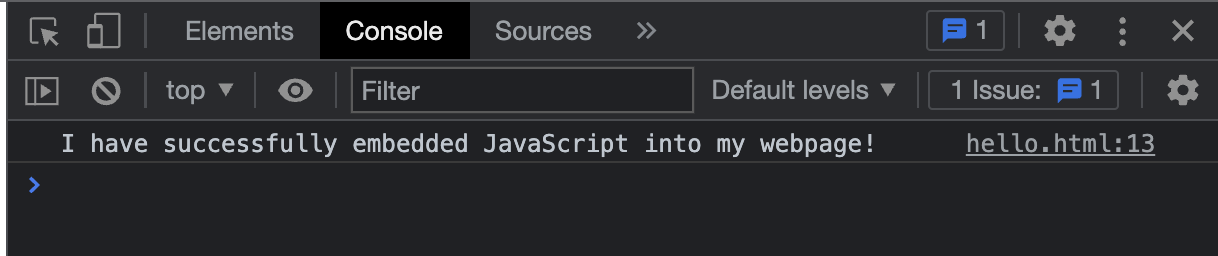
\includegraphics[width=0.5\textwidth]{Images/embedding3.png}
    \caption{Web-page's console}
    \label{fig:screenshot}
\end{figure}

I then sought to learn how to create functions in JavaScript. I started with simple functions that perform basic tasks, such as adding two numbers together or printing a message to the console. This helped me get comfortable with the syntax and structure of functions in JavaScript. After overcoming the basics, I explored more advanced topics, such as function hoisting, closures, and callbacks. These concepts helped me write more powerful and flexible code.

I began solving challenge questions in JavaScript (Figure 4. There are more functions that I created in my GitHub repository in \emph{functions.js}). I was stumped at the start because the challenges required JavaScript methods to solve that I was unaware existed. Every time I looked at a solution and stumbled across a new method, I was forced to research more about it to understand how it is used. 

The function I created in Figure 4 works as follows: Given an array filled with object ID's, the function returns a list of unique ID's in a string. For this problem, I learnt how to use the map method that calls a provided callback function, how to use the JavaScript spread operator, and how to effectively convert an array to string with comma separated values.

The challenge questions helped identify areas where I needed to improve my understanding of the language, allowing me to focus my learning efforts more effectively. Watching a video and completing interactive challenges was an engaging and interactive way to learn, keeping me motivated and interested in the material. By completing challenge questions and seeing my progress, I built confidence in my ability to write JavaScript functions and tackle increasingly complex problems.

\begin{figure}[ht]
    \centering
    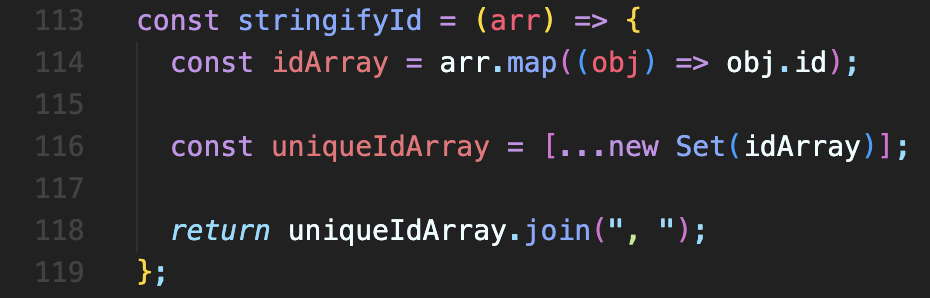
\includegraphics[width=0.5\textwidth]{Images/functions.png}
    \caption{JavaScript challenge question that I solved while learning how to create functions}
    \label{fig:screenshot}
\end{figure}

The final thing left to learn for Level A was scoping. I had covered some of this whilst learning about functions, but sought a more comprehensive understanding of the topic. 

I mainly read documentation and watched videos to understand this concept, and tried different things out myself. I built varying nested structures, and ran my code to see the output in the console. I compiled notes in my \emph{scope.js} file of my findings. Figure 5 shows a snippet of my notes on scope in JavaScript. I investigated Lexical Scoping, Vairable Shadowing and Leaked Globals. 

\begin{figure}[ht]
    \centering
    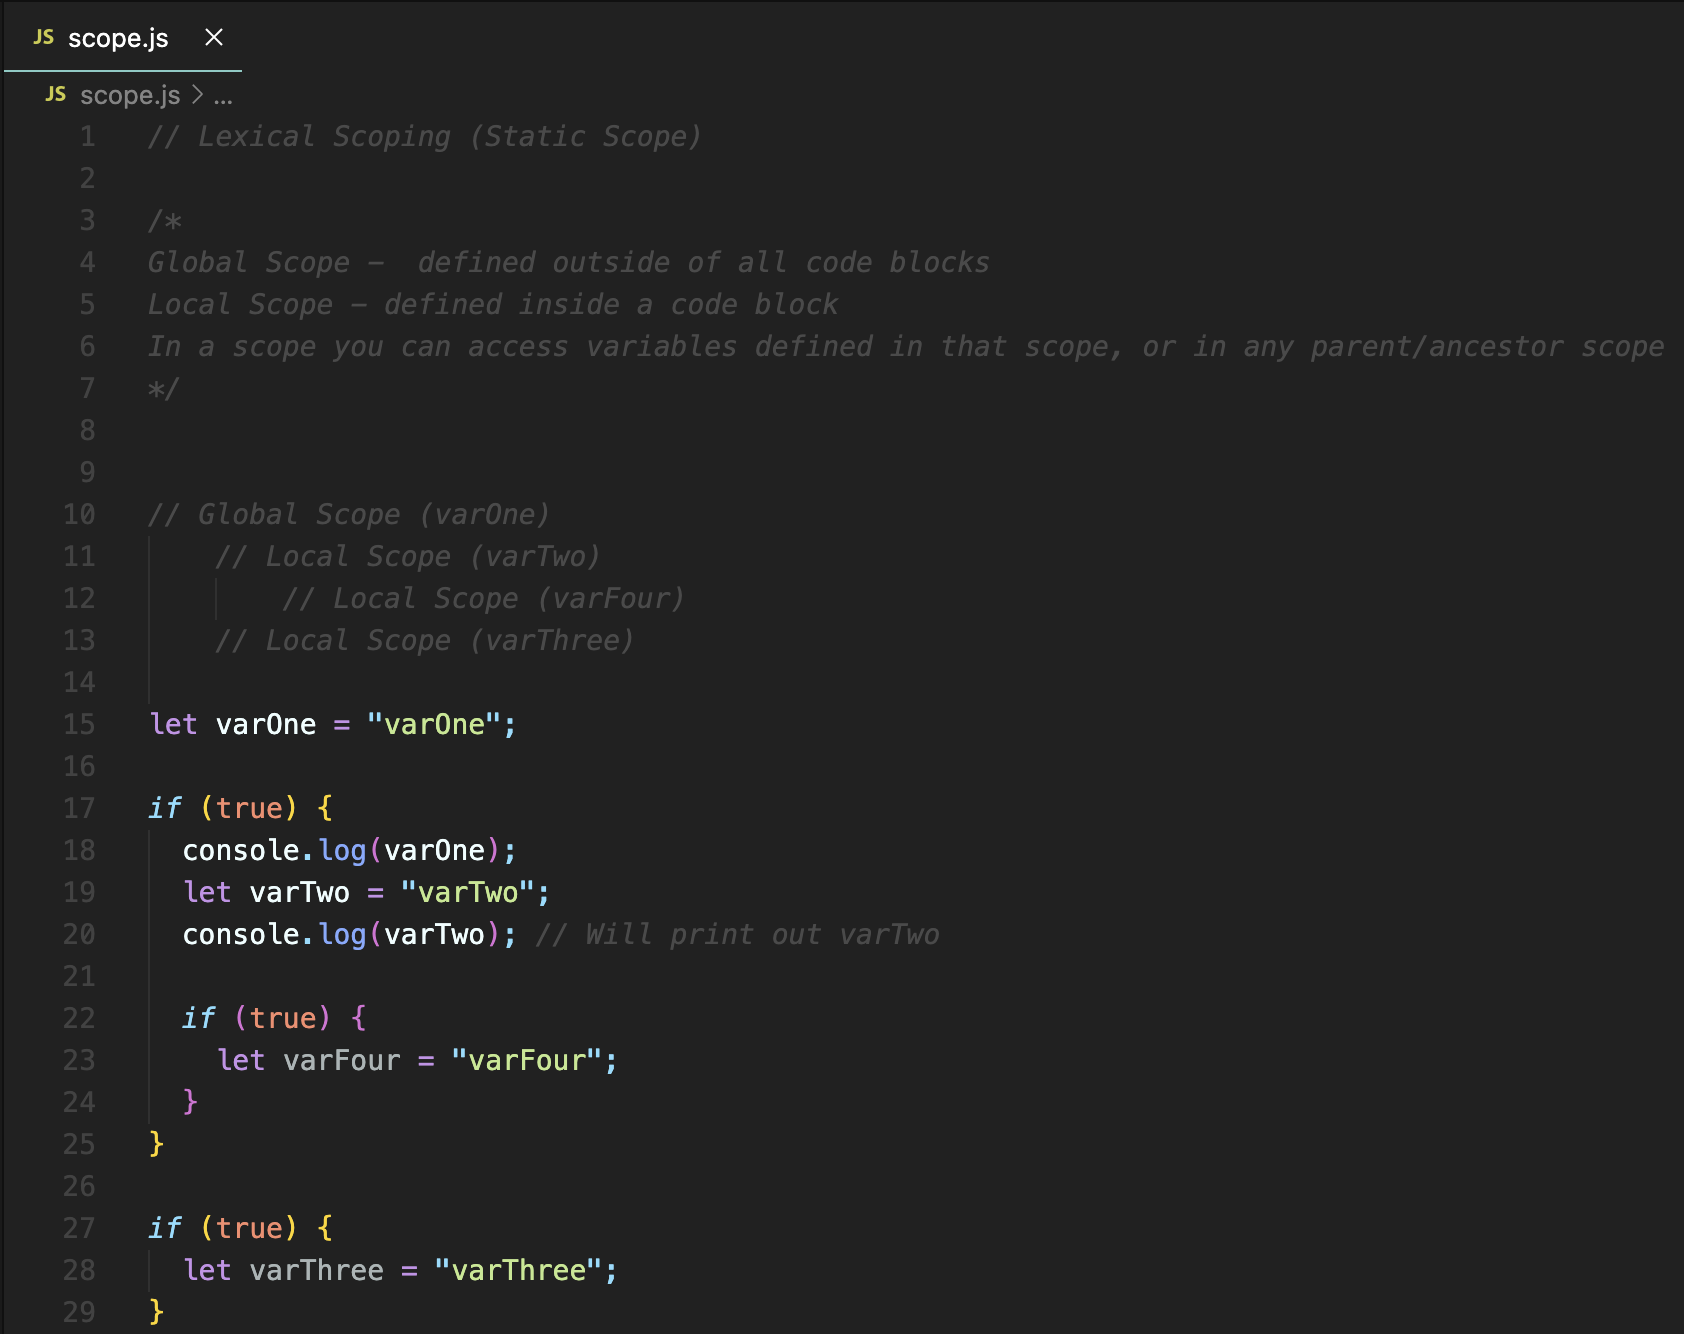
\includegraphics[width=0.8\textwidth]{Images/scope.png}
    \caption{My notes on JavaScript Scope}
    \label{fig:screenshot}
\end{figure}

%=============================================================================

\newpage
\section{Level B: Basic Application}

\subsection{Level B Demonstration}

The key concepts demonstrate for Level B are:

- Embedding JavaScript into a web-page

- JavaScript functions

- Accessing web-page elements

- Event-based triggers

I have incorporated all of these concepts to create a counter. My application involves a HTML structure for the counter, including buttons to increment and decrement the counter and a place to display the current count (embedding JavaScript into a web-page, accessing web-page elements). I added JavaScript code to listen for button clicks and update the counter accordingly (event-based triggers, functions). I added additional CSS to style my counter application.

\subsection{Application artifacts}

I created a simple counter application using JavaScript embedded into a web-page. The application displays the current count on the page and provides three buttons: Increment, Decrement, and Reset. The user can interact with these buttons to manipulate the counter value (Figure 6).

Here's how it works and how I created it:

First I created the basic HTML structure with a heading, a paragraph to display the count, and three buttons with unique id attributes for incrementing, decrementing, and resetting the counter. I was able to access these web-page elements using their id attributes (Figure 7). The JavaScript \emph{getElementById()} returns a reference of the element whose id property matches the specified string. 

I then added JavaScript code by having a separate \emph{app.js} file that is referenced in the HTML code using a <script> tag. JavaScript is required to handle the functionality of the counter.

I initialised a variable \emph{count} to store the current counter value, starting at 0. The function \emph{updateCounterDisplay()} sets the \emph{innerHTML} of the \emph{counterDisplay}y element to the current value of \emph{count}.

I added event listeners to the buttons for handling user interactions (Figure 8). These click-based event listeners are responsible for changing the value of of \emph{count}. The variable is either incremented by one, decremented by one, or reset to 0, depending on the button clicked by the user.

The resulting application is a simple, interactive counter that allows users to increment, decrement, or reset the count using the corresponding buttons. The count value is displayed on the page and is updated. I added CSS to make the application aesthetically pleasing.

\begin{figure}[ht]
    \centering
    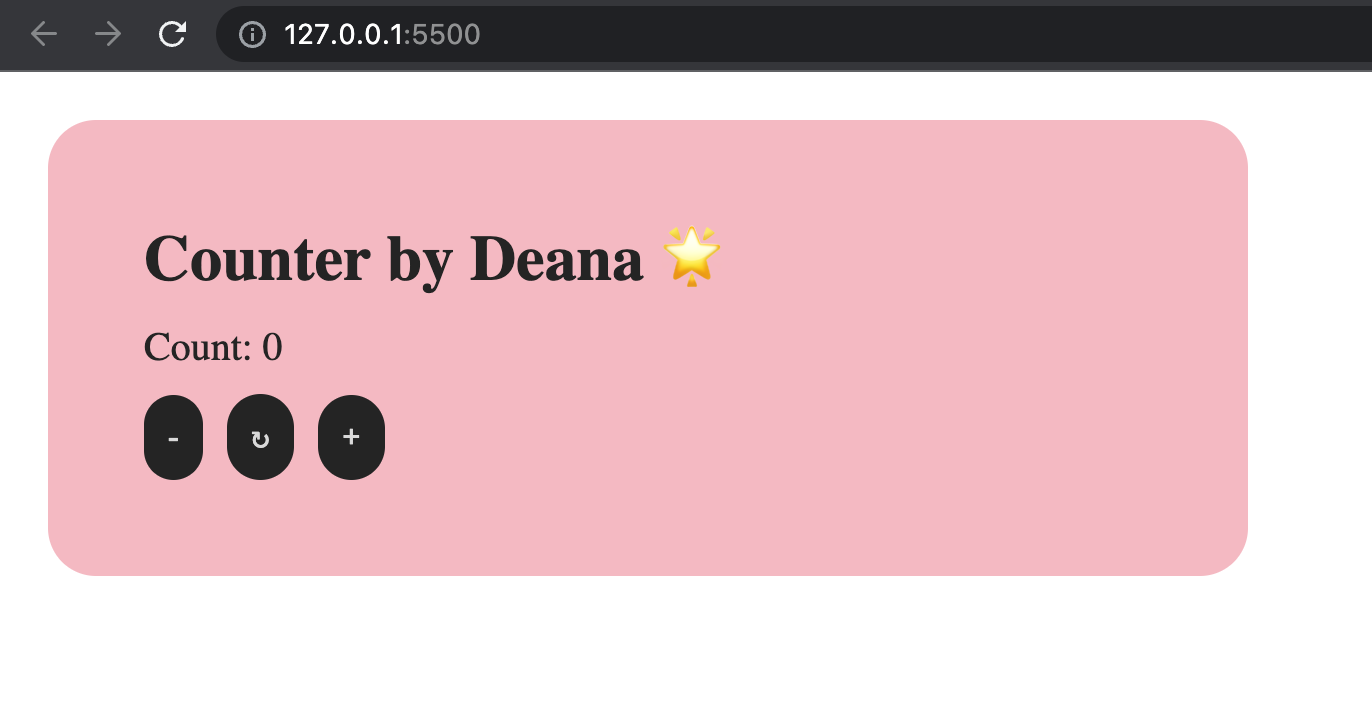
\includegraphics[width=0.8\textwidth]{Images/counter1.png}
    \caption{Counter Interface}
    \label{fig:screenshot}
\end{figure}

\begin{figure}[ht]
    \centering
    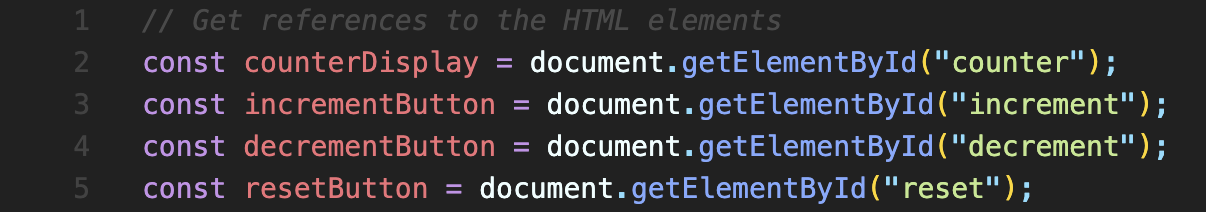
\includegraphics[width=0.8\textwidth]{Images/counter2.png}
    \caption{Accessing web-page elements}
    \label{fig:screenshot}
\end{figure}

\begin{figure}[ht]
    \centering
    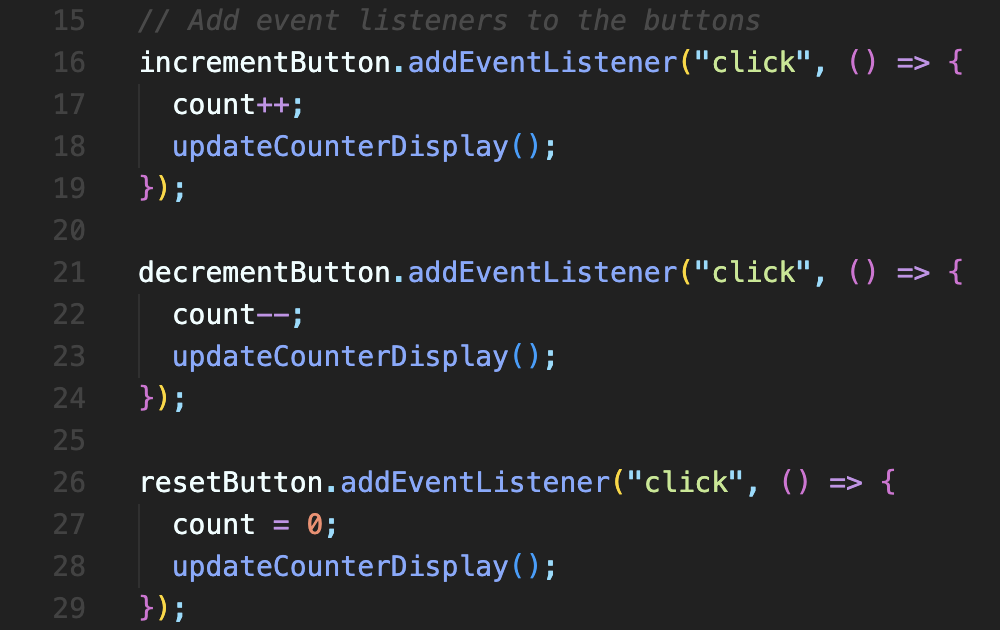
\includegraphics[width=0.8\textwidth]{Images/counter3.png}
    \caption{Event-based triggers}
    \label{fig:screenshot}
\end{figure}

%=============================================================================


\newpage
\section{Level C: Deeper Understanding}

\subsection{Strengths}

 JavaScript is versatile in nature, which enables developers to create dynamic and interactive web applications. As Ian Deed (2023) states "JavaScript has been the single most popular programming language worldwide for some time now." \cite{PangeaBestPractices}. Being lightweight and effective, allowing event-driven and asynchronous programming, and having a wide ecosystem with a variety of libraries and frameworks are some of JavaScript's key strengths. In addition, JavaScript may be used for full-stack development because it can be executed on both the client and server side (using Node.js).

\subsection{Weaknesses}
Even though it is so popular, JavaScript has certain drawbacks. Because it is not a strictly-typed language, it may exhibit unpredictable behaviour and have elusive bugs. Additionally, the language lacks some capabilities available in other programming languages, such as appropriate multithreading support and namespaces, which can make developing large-scale applications more difficult. Furthermore, due to its client-side execution, JavaScript may run less quickly than languages that are compiled and raise security issues. Tutorials Point highlights this security issue, explaining that the user can see the JavaScript code \cite{TutorialsPointAdvDisadv}. This creates a potential of misuse, whereby code is added to a website that compromises the security of data sent through the website.

\subsection{Usefulness}
A highly interactive and aesthetically pleasing e-commerce website for businesses can be created using JavaScript. Developers may construct responsive and captivating user interfaces that improve the shopping experience. This is done by combining JavaScript's frontend capabilities with libraries and frameworks like React or Angular. JavaScript enables the seamless implementation of features like product filters, real-time inventory updates, and customised suggestions. This improved user experience can increase user engagement, customer happiness, and ultimately conversion rates, which can raise revenue for the business.

\subsection{Key Question 1}
JavaScript should be used for interactive web applications, as the programming language excels at building dynamic and interactive web applications, where user interactions or real-time updates are essential. It should also be used in full-stack development, as using JavaScript and NodeJS allows developers to use the same language for both frontend and backend, simplifying the development process. On the other hand, JavaScript should not be used for static websites. If a website is static and doesn't require user interaction, JavaScript may not be necessary, as HTML and CSS can suffice. Due to the aforementioned security concerns, JavaScript should also not be used in security-sensitive applications, as the code can be easily viewed and manipulated on the client side. 


\subsection{Key Question 2}
Because they offer reusable code, structure, and best practises, JavaScript frameworks streamline and speed up web development. As well as imposing a particular design to promote organisation and maintainability, they include built-in components and utilities for quickly building complicated features with little code. Angular, React, Vue, Ember, and Backbone are some popular JavaScript frameworks. These frameworks, created with JavaScript, increase its functionalities and allow programmers to create web applications more quickly while meeting particular requirements and providing particular benefits.

%=============================================================================

\newpage
\section{Level D: Evolution of skills}
\vspace{5mm}
\subsection{Level D Demonstration}

I developed an interactive Tic Tac Toe game using HTML and CSS to build the interface, and JavaScript to handle the game's logic and interactivity. The game features a 3x3 grid where two players, X and O, take turns clicking on the squares to make their moves. The game displays the current player's turn, detects wins or draws, and allows users to restart the game at any time. 

\subsection{Application artifacts}

The Tic Tac Toe application I created is a web-based game that allows two players to play against each other, with one player using 'X' and the other using 'O'. It has a 3x3 grid layout, and the objective is to get three of the same symbols in a row, either horizontally, vertically, or diagonally.

I began by setting up the HTML structure with the basic layout of the game: a title for displaying the current player's turn, a 3x3 grid of buttons as the game board, and a "Restart Game" button (Figure 9). Using CSS, I styled the game board, squares, and restart button. The boardwrapper class defines the width and height of the game board, while the boardsquare class styles individual squares, setting their dimensions, background color, font size, and cursor style. The restart class styles the "Restart Game" button.


\begin{figure}[ht]
    \centering
    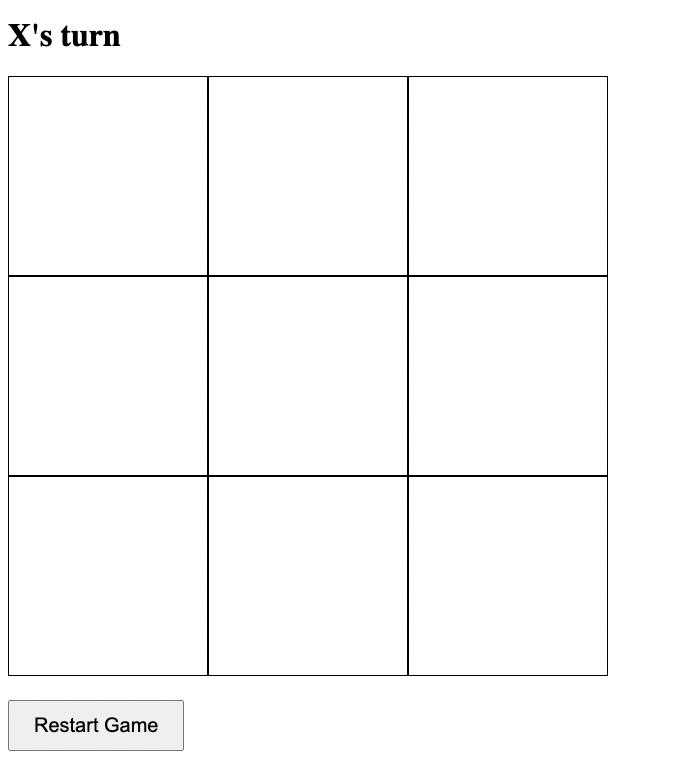
\includegraphics[width=0.3\textwidth]{Images/ttt1.png}
    \caption{Game interface}
    \label{fig:screenshot}
\end{figure}

I then began to introduce JavaScript to make the game interactive. I initialised game variables to track the current player (currentPlayer), the game's status (gameOver), and the board's state (board). I also selected all the squares on the board using querySelectorAll (Figure 10).

\begin{figure}[ht]
    \centering
    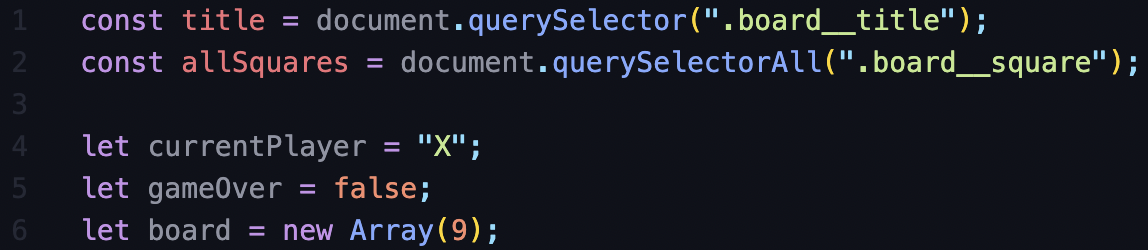
\includegraphics[width=0.6\textwidth]{Images/ttt2.png}
    \caption{Initialising game variables}
    \label{fig:screenshot}
\end{figure}

The next section of my code was the most important, and handled all the game logic. I had to be very careful about the logic flow of my program. Firstly, I added click event listeners to every square of the board using the forEach method. Since "board" is an array of length nine, and there are nine squares, each index of the "board" array maps to a corresponding square. This is important for calculating which player has won (Figure 11).

\begin{figure}[ht]
    \centering
    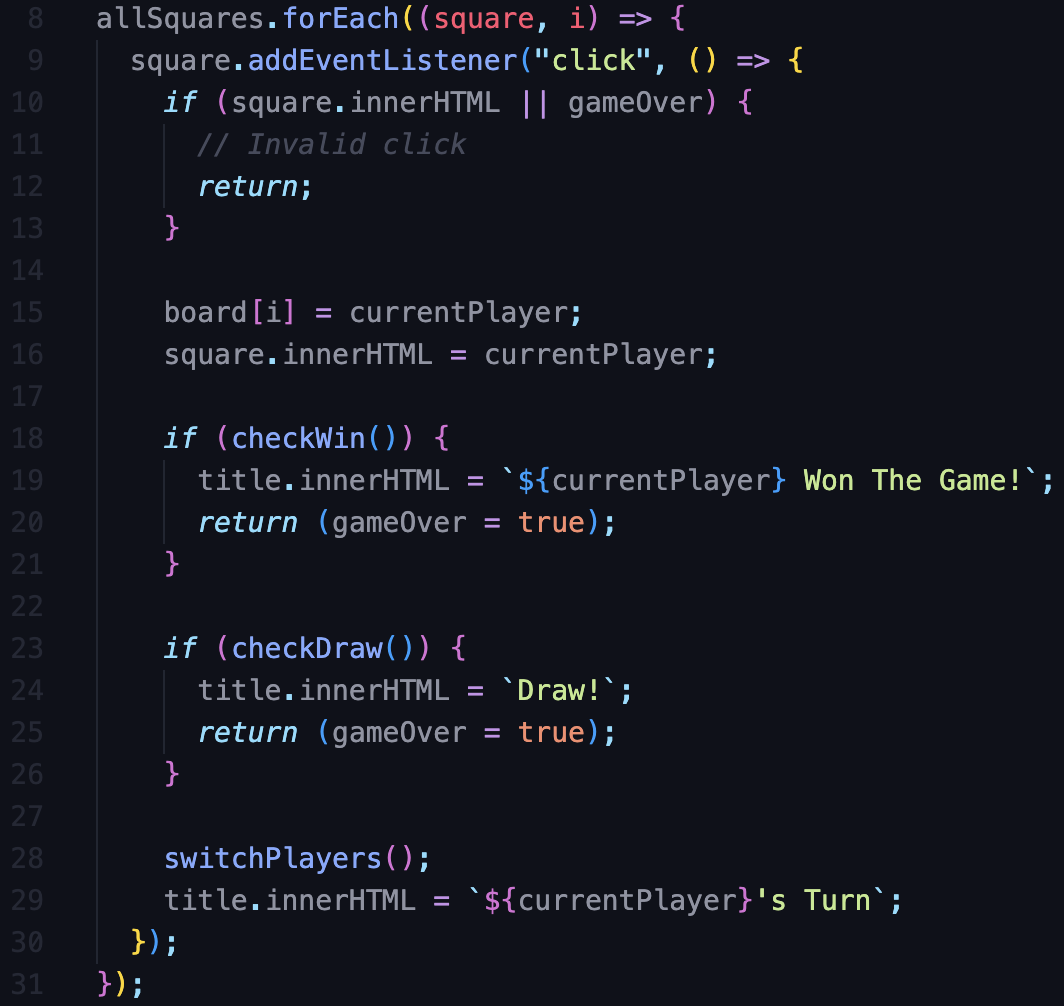
\includegraphics[width=0.6\textwidth]{Images/ttt3.png}
    \caption{All logical game conditions}
    \label{fig:screenshot}
\end{figure}

When a square is clicked, the board state and display are updated (line 15-16 in Figure 11). The script updates the board array with the current player's symbol at that position "board[i]" and displays the symbol in the clicked square using "square.innerHTML = currentPlayer".

When I tested my game, I discovered I needed to account for two edge cases. I considered the case where a player selects a square that has already been chosen. The game board should NOT override the new selection. Further, if a game is a draw, and there are empty squares remaining, they should not be clickable. To allow this to work, the callback function for the event checks if the clicked square is empty and if the game is still ongoing before making a move. This is reflected in line 10-13 in Figure 11.

I also handled switching players after every turn, and updating the title display to reflect the current player's turn (line 28-29 in Figure 11). The switchPlayers function toggles the current player between 'X' and 'O' by using a ternary operator: "currentPlayer = currentPlayer === 'X' ? 'O' : 'X';"

I then worked on the checkWin function (Figure 12). The checkWin function checks for a winning combination using an array of winning index sets (winningIndicies). It iterates through these sets and compares the symbols at those indices on the board. If the symbols match and are not undefined, the function returns true, indicating a win. 

Checking if the symbols are undefined was a crucial step in the logic of my code. Initially, the board array is of length 9 and undefined in every slot. This would mean the symbols would be equivalent in a winning combination, and wrongfully return true. Therefore, it is important to check if a square is populated, and that the matching symbols aren't a result of empty squares.

\begin{figure}[ht]
    \centering
    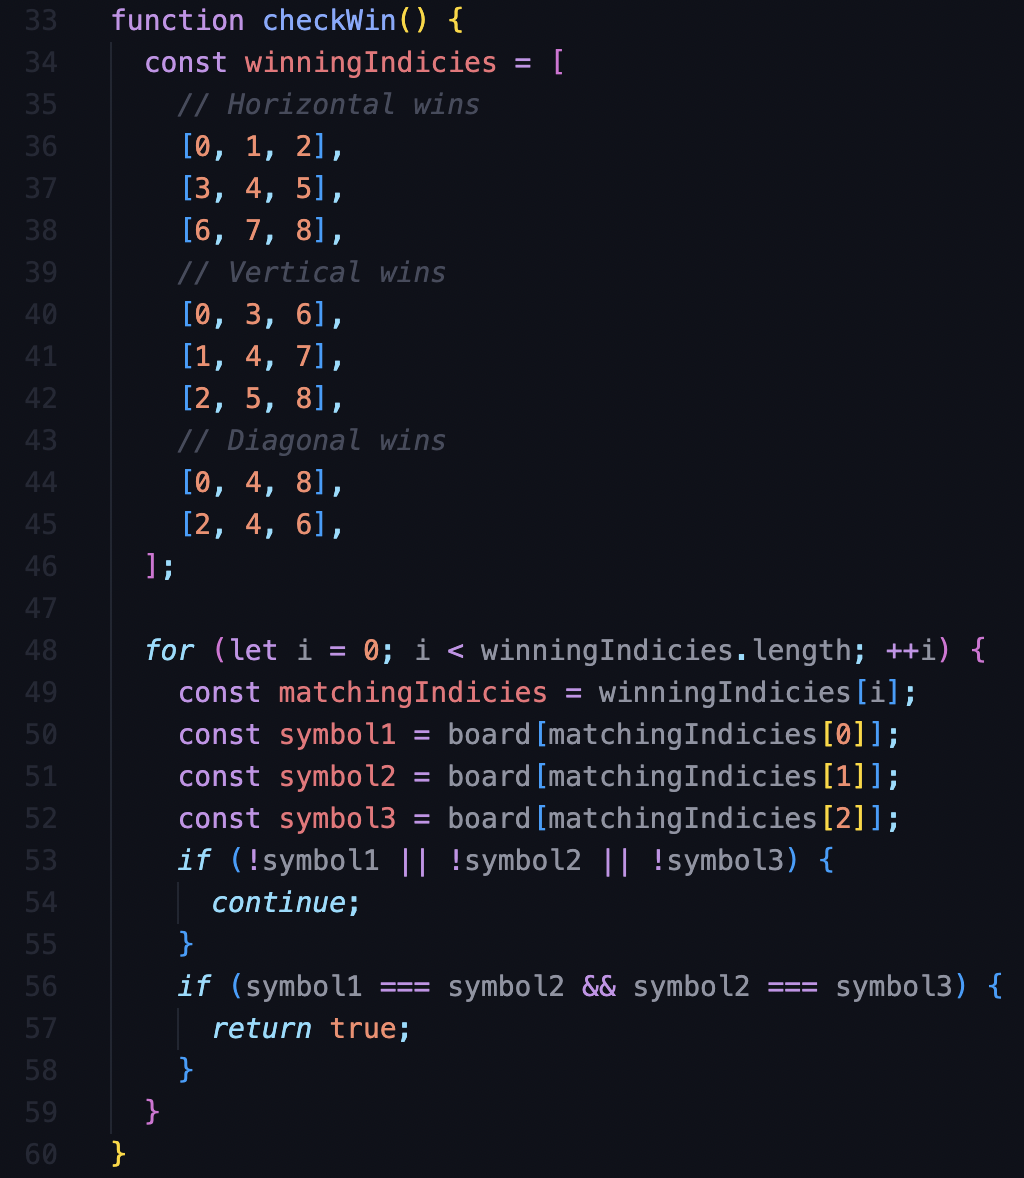
\includegraphics[width=0.6\textwidth]{Images/ttt4.png}
    \caption{Function to check if a win has occured}
    \label{fig:screenshot}
\end{figure}

If there is a win, the board's title is updated to reflect this (Figure 13), and the gameOver state is set to true, to ensure no more squares can be clicked. 

\begin{figure}[ht]
    \centering
    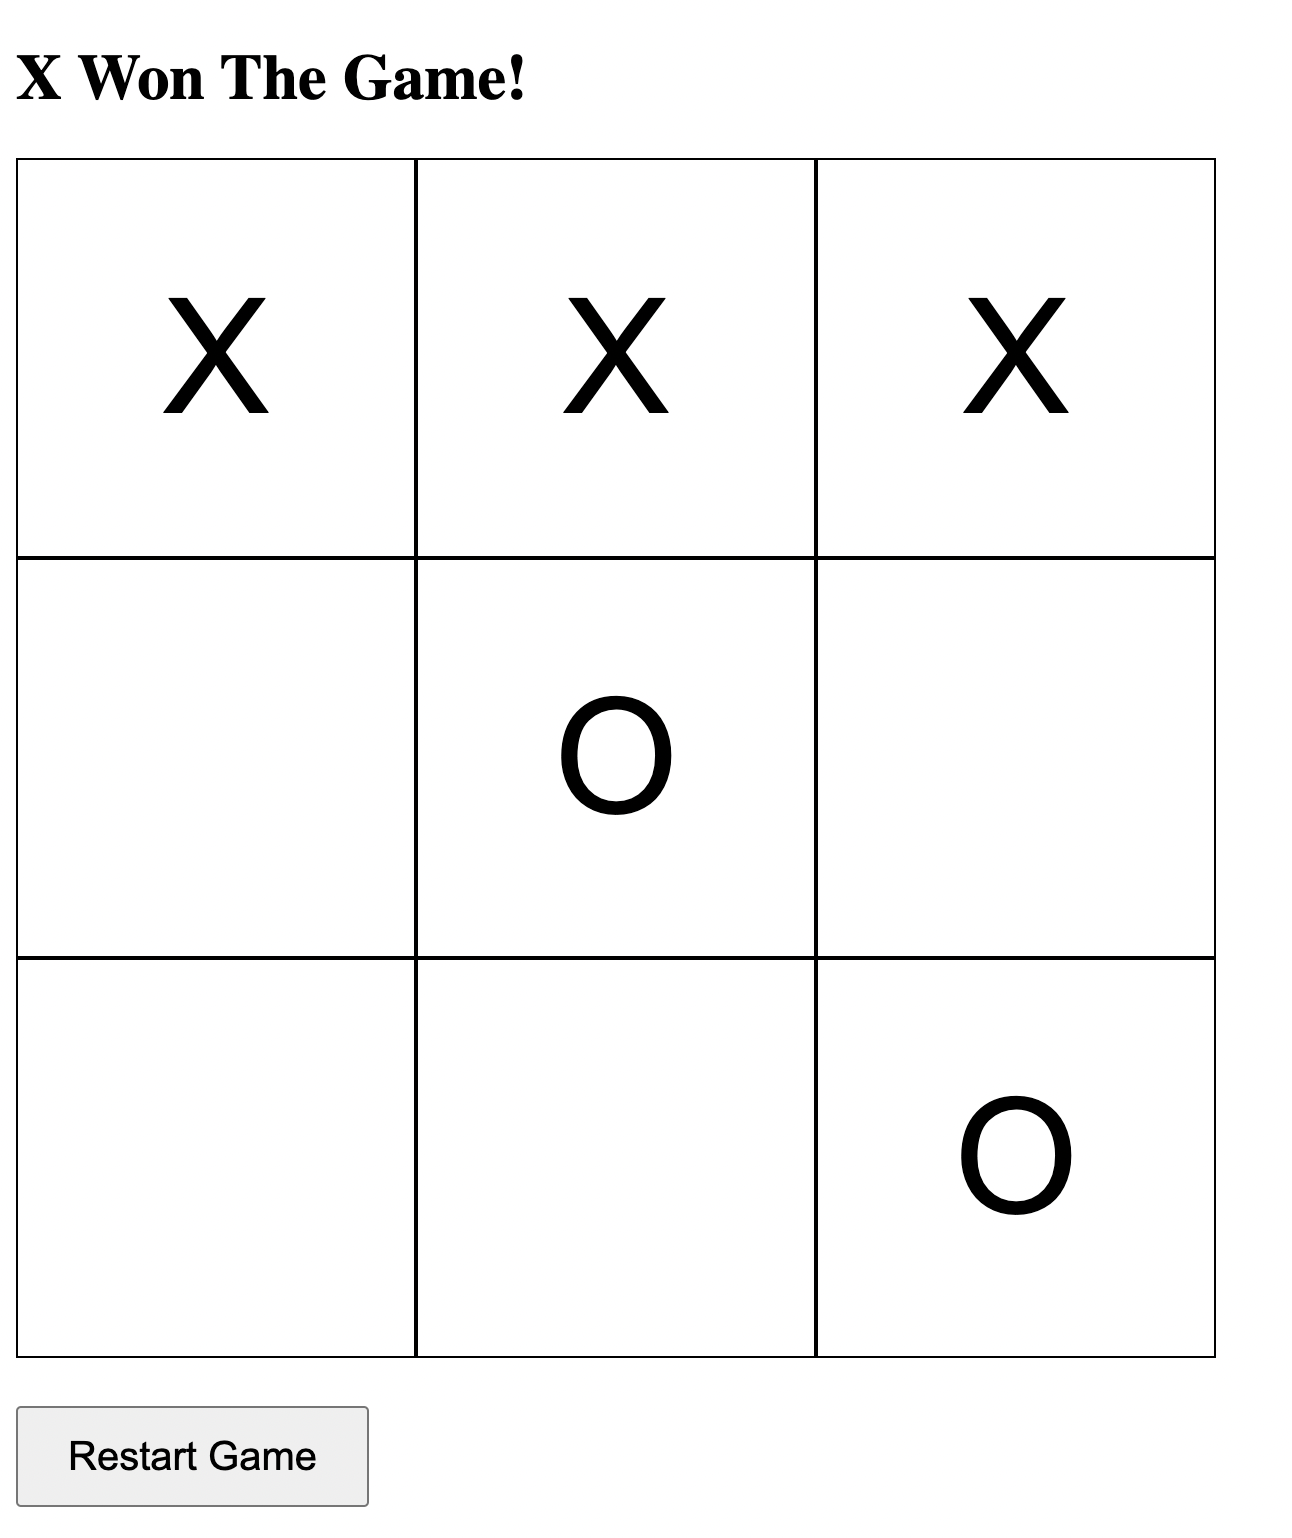
\includegraphics[width=0.3\textwidth]{Images/ttt5.png}
    \caption{Board title changing to reflect X's win. No other squares can be clicked}
    \label{fig:screenshot}
\end{figure}

Checking if there is a draw was more straightforward. The checkDraw function checks if all squares on the board are filled by iterating through the board array. If it finds an undefined value, it returns false. Otherwise, it returns true, indicating a tie (Figure 14). It is important to check this condition only once we know there has not been a win, as it is possible to win with a filled board. If a draw has occured, the board title is updated (Figure 15).

\begin{figure}[ht]
    \centering
    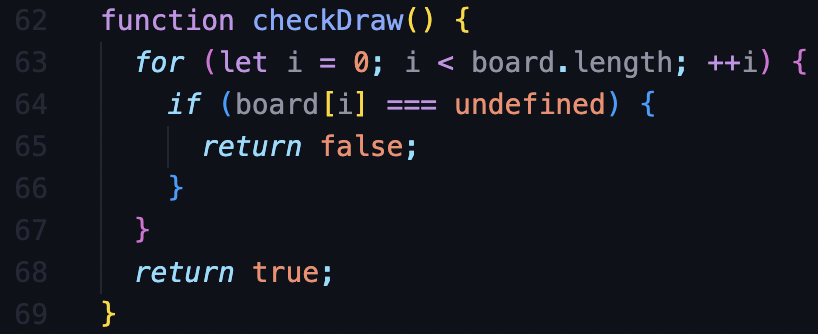
\includegraphics[width=0.6\textwidth]{Images/ttt6.png}
    \caption{Function to check if a draw has occured}
    \label{fig:screenshot}
\end{figure}

\begin{figure}[ht]
    \centering
    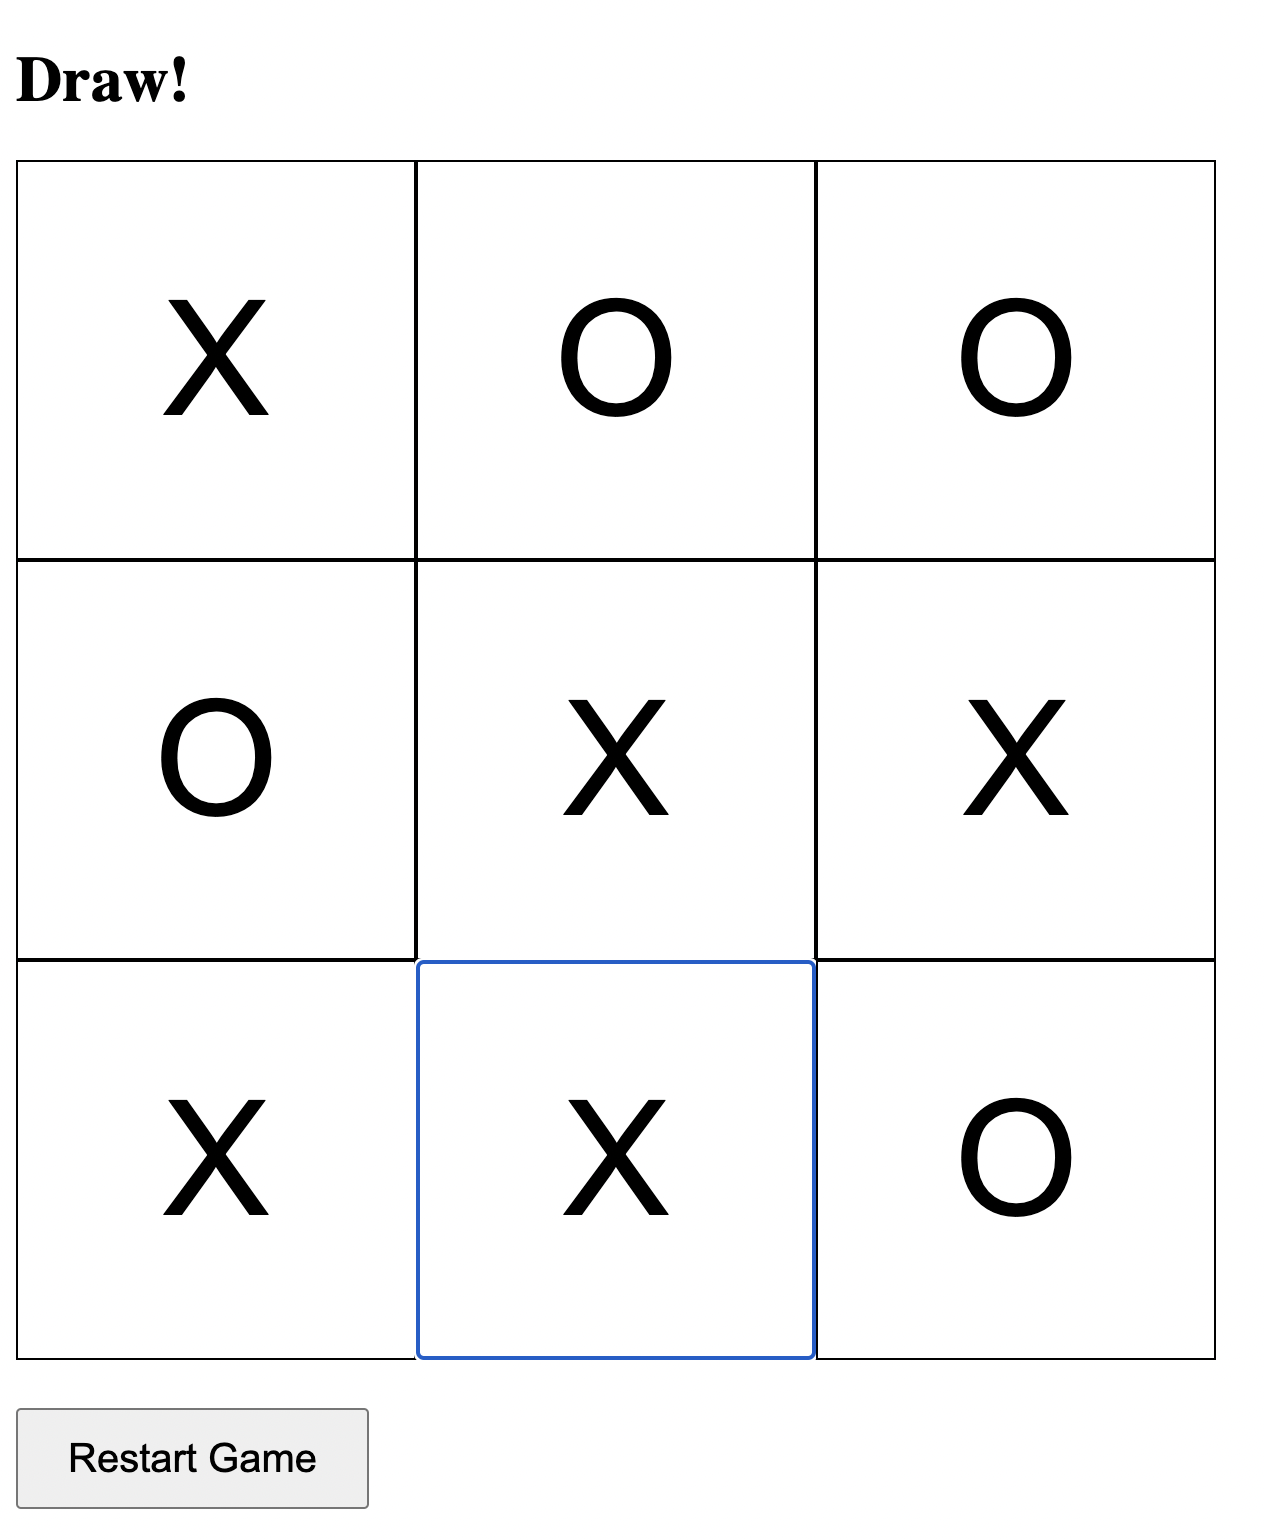
\includegraphics[width=0.3\textwidth]{Images/ttt7.png}
    \caption{Board title changing to reflect a draw}
    \label{fig:screenshot}
\end{figure}

The final thing to consider is restarting the game. The "Restart Game" button has an onclick attribute that triggers the restartGame function. This function resets the gameOver variable, creates a new empty board array, clears the square content, and updates the title display to show the current player's turn (Figure 16).

\begin{figure}[ht]
    \centering
    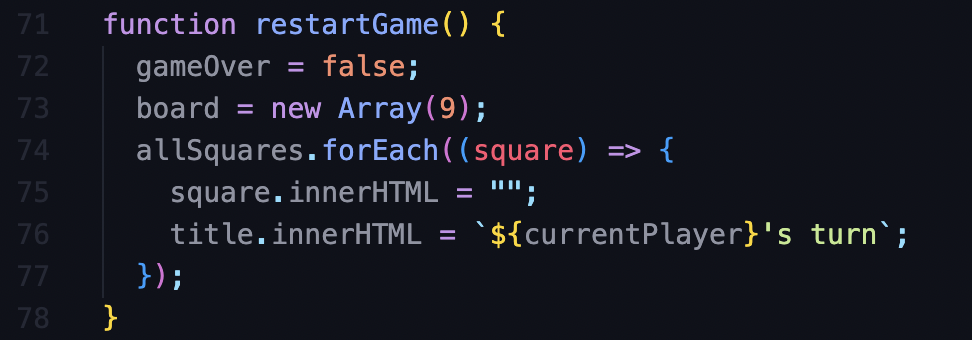
\includegraphics[width=0.6\textwidth]{Images/ttt8.png}
    \caption{Function to restart the game}
    \label{fig:screenshot}
\end{figure}

\subsection{Alternative tools/technologies}

Two alternative tools/technologies to JavaScript for developing a Tic Tac Toe game are Python (with a web framework like Flask) and TypeScript.

\subsection{Comparative Analysis}

Python (with Flask): The Python web framework Flask can be used to build lightweight web applications. Python with Flask may be prefered over JavaScript in circumstances where a developer has a strong foundation in Python and wishes to use only one language for both backend and frontend development. Real-time communication can be achieved by using a library like Flask-SocketIO, making it simpler to create multiplayer games. Python is also well suited for rapid prototyping and development because to its extensive ecosystem of libraries and readability.

TypeScript: TypeScript is a statically-typed superset of JavaScript that adds optional type-checking to the language.  TypeScript may be prefered over JavaScript in circumstances when a bigger-scale Tic Tac Toe game is being developed, such as one with sophisticated features, complex logic, or a component of a larger programme. Static typing in TypeScript can aid in the early detection of type-related mistakes, enhancing the dependability and maintainability of the code. Other developers will find it simpler to comprehend and contribute to the codebase thanks to the improved code readability and IDE support provided by the extra type information.

However, because it is natively supported by web browsers without the need for any additional tools or plugins, JavaScript is a fantastic option for smaller projects or for addressing a wide range of browsers and devices. Because of its adaptability and dynamic character, it also permits rapid development and iteration.
%=============================================================================

\newpage

\bibliographystyle{IEEEtran}
\bibliography{main}

\end{document}
\end{report}
